\chapter{Evaluation}
\label{sec:evaluation}

The main issue of the current implementation in Bdrive is the poor scalability of the number of file keys. For each new device, a new file key needs to be created and maintained. The proposed prototype serves as the proof-of-concept that such a distributed, secure system can exist and which in addition fits all the requirements of section \req{sec:requirements} and scales better than the current system implemented in Bdrive. 

To stress this thesis, different benchmarks will be conducted to compare the proposed prototype to a similar environment such as Bdrive. The goal of this section will be to show that following assumption holds true:

\begin{center}
\textit{The ABE-based solution of the in section \ref{sec:implementation} proposed system to solve the scalability problem of a secure cloud storage system, scales at least as good as the RSA-based approach, described in section \ref{sec:background}, regarding the number of file keys that need to be maintained.}
\end{center}

While this assumption should hold true for all group operations the performance of thous operations need to be taken into account as well. The goal is to find the number of attributes per user, at which \name performs at least as good as the RSA-based sibling. It is expected that such a number can be found for encryption and member join operations. But when it comes to member leave operations, it is expected that there is no configuration in which the proposed prototype performances better then the RSA solution, due to additional shared-key managed and complex revocation mechanism. 

\section{Upper-Bound and Worst-Case Scenario}
\label{sec:upper-bound-and-worst-case-scenario}
In this section it will theoretically argued why \name scales at least as good as the current solution for secure cloud storage systems. The number of file-keys scale in a ratio of one-to-one with the number of "OR"-gates $+ 1$\footnote{A file key need to be created for the left and right sub-tree respectively. Having an access policy with one "OR"-gate will case the creation of two file keys.} in the access policy as described in section  \ref{sec:extension-to-dnf-policy}. The maximal number of "OR"-gates in an access policy would be to mention each user in the group explicitly. Such a policy looks like the following example:

\begin{center}
\begin{lstlisting}[caption={Worst case access policy. The used email address is a unique attribute per user.},captionpos=b]
(alice@example.com OR bob@example.com OR ... OR zara@example.com)
\end{lstlisting}
\end{center}

It does not make sense to include more "OR"-gates into this policy since it would represent redundant information. The number of files keys per $n$ user scale with $O(n)$ (same way as Bdrive) in \name if and only if, no suitable subset of district attributes of any two users can be found so that the $n$ users can be described with $o < n-1$ "OR"-gates $o$. 
That means if at least $k$-users, with $k > 1$  can be completely described by an AND-policy, the number of file keys needed will shrink to $n – k +1$ file keys. Each "OR"-gate that can be substituted by "AND"-gates reduces the number of file keys. 
If that is not the case, say no user share the same attribute, for each user an unique attribute needs to be used (for example the email address of the user) which is embedded in an inclusive attribute policy. 

Analogous, the best access policy that can be constructed would be one using only "AND"-gates resulting in only one file-key regardless of the number of embedded attributes. This behavior is inherited from  TF-DAC-MACS where it is possible to embed any number of attributes in an disjunctive condition into one file-key. 

\section{Performance and Scalability Analysis}

To evaluate the performance and scalability of \name against the RSA-based implementation different benchmarks are conducted. While the main focus remains on reducing the number of file keys for group operations, it is also important to measure the performance of encryption, member join and member leave actions. In the following sections each of the three different actions will be evaluated and an expectation about the experiment outcome will be given.

The benchmark evaluation is executed on a Server machine utilizing 6 vCPU cores (Intel(R) Xeon(R) CPU E5-2680 v3 @ 2.50GHz, 30MB cache size), 12 GB RAM and running on Ubuntu 16.04 LTS 64bit. For the evaluation OpenJDK 1.8.0\_191 is used. Each of the benchmark does not spawn any threads or uses parallelism. \footnote{Single thread assumption is based on the implementation of \name. This assumption must not hold true for libraries that are used under the hood for RSA and AES cryptography (bouncycastle 1.60) or pairing-based cryptography (jPBC 2.0.0).}  For pairing operations the native PBC extension is used. \footnote{\url{https://crypto.stanford.edu/pbc/}} 

Each benchmark averaged over 25 executions. Still artifacts and noise may occur, casing spikes or sudden outliers. Before each benchmark a warm-up phase is executed to fill caches and optimize branch predictions. However, it is still possible graphs become linear decreasing over time. Such behavior can only be traced back to optimized caches and less left-over artifacts from the initialization process.

\subsection{Encryption}
Encryption is the most interesting topic to evaluate since it scales using RSA with the number of users and using ABE with the number of attributes. With having the assumption of section \ref{sec:comparing-secure-group-communication-to-attribute-based-encryption} in mind, that states that the number of attributes is smaller or equal to the number of users in the shared group, ABE should be able to archive a better performance. 

\subsubsection{Expectation}
Classical encryption that uses RSA to encrypt the file key asymmetrically scales with the number of key-identities, in the following entitled users. For each new file in the group a suitable file key for each user must be created. The resulting assumption is that the RSA based approach scales linearly with increasing number of users. Same holds true for the cipher text size, which describes the aggregated sum of all file keys for one file. The number of file keys should scale on the order of 1-to-1 with the number of users. 

In contrast to that stands \name. It scales with the number of attributes per cipher text rather then the number of users. Given this assumption an intersecting point of "attributes per user" can be calculated where \name scales better then the RSA approach. Where this intersecting point is located depends on the number of attributes, number of users, the chosen policy and the computing power of the executing machine. At some point the access policy can get so large that the prototype solution will have to advantage regarding the computation time. 

\subsubsection{Benchmark: "AND"-Policy}
There where two different scenarios evaluated. The and-policies (best-case) and then the or-policies (worst-case) are analyzed independently from each other for performance and scalability. The benchmarks are performed over an increasing number of users. For each $n$ users a new attribute is introduced. The notation of $a$-for-$n$ defining $a$ as the number of attributes \textit{for} $n$ users. The benchmark is evaluated for the configurations $1$-for-$\infty$, $1$-for-$1$, $1$-for-$2$, $1$-for-$4$, $1$-for-$5$. Given the number of users the attributes can be calculated in the following way: $\lfloor \frac{n}{a} \rfloor$. 

% picture
\begin{figure}[!t]
\centering
    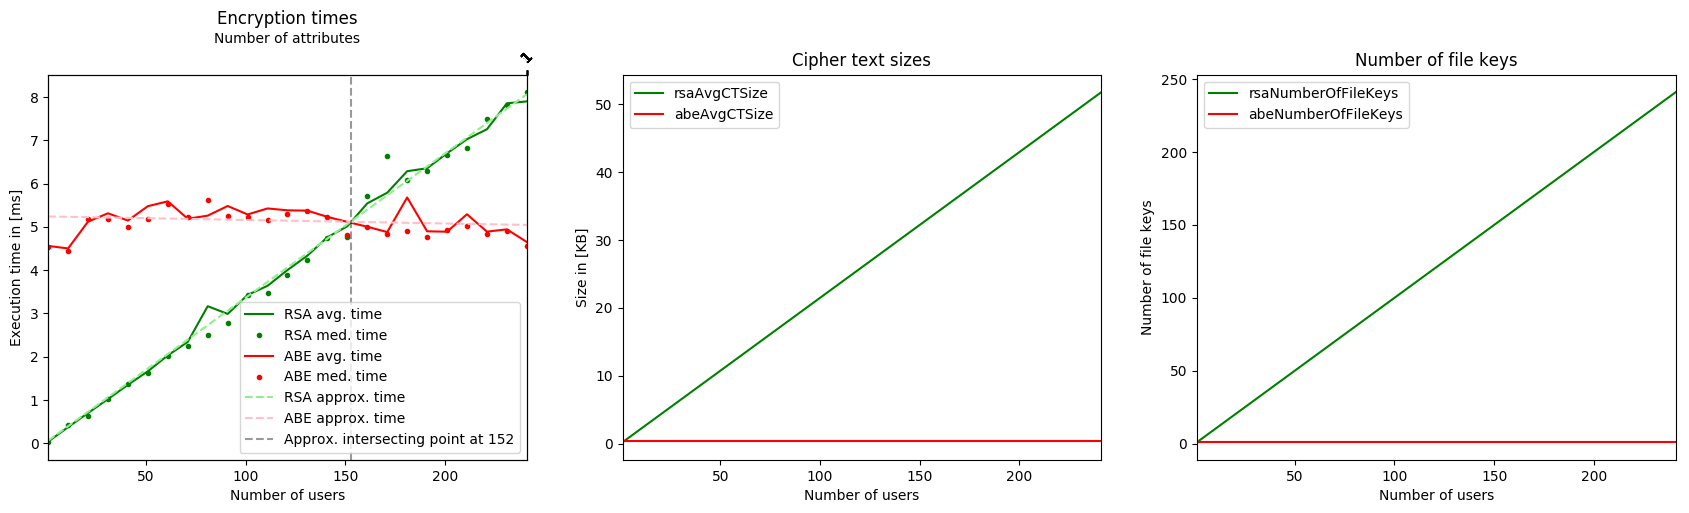
\includegraphics[width=\linewidth]{img/eval-and-policy/encrypt_incrementing_10.png}
    \caption{$1$-for-$\infty$ configuration using "and"-policy}
    \label{fig:1-for-infty-and}
\end{figure}
\begin{figure}[!t]
\centering
    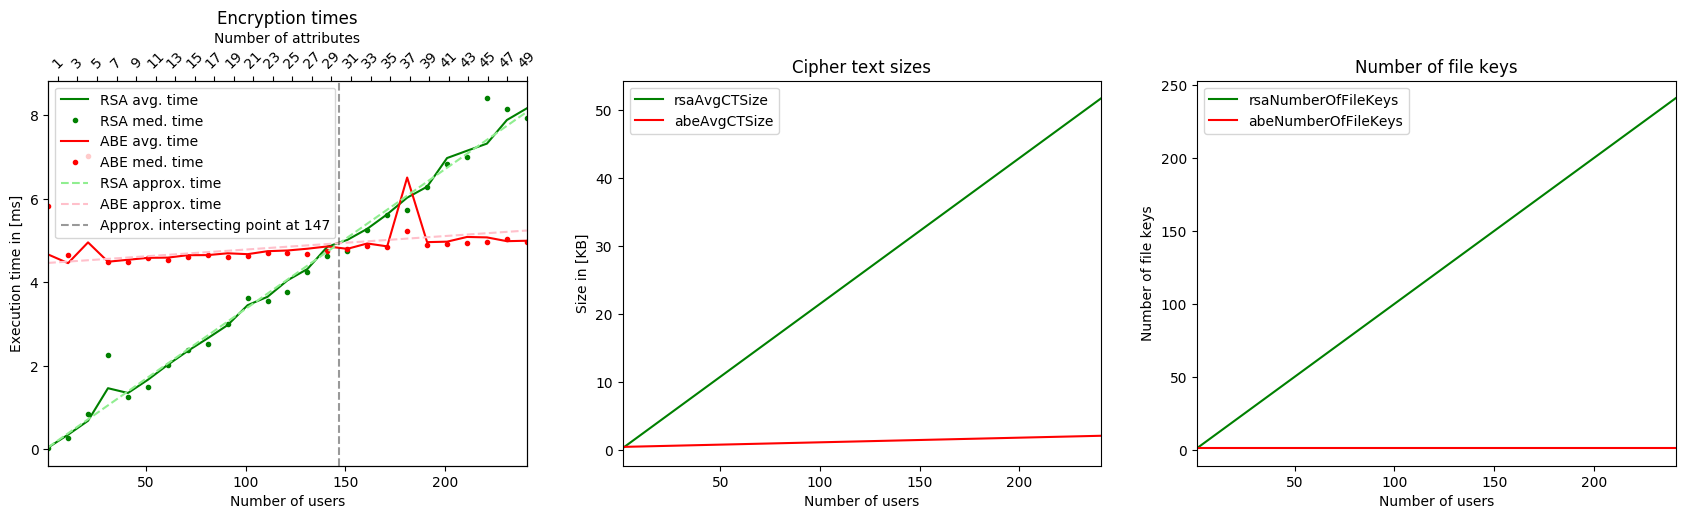
\includegraphics[width=\linewidth]{img/eval-and-policy/encrypt_incrementing_10_attribute_increment_1per5User.png}
    \caption{$1$-for-$5$ configuration using "and"-policy}
    \label{fig:1-for-5-and}
\end{figure}
\begin{figure}[!t]
\centering
    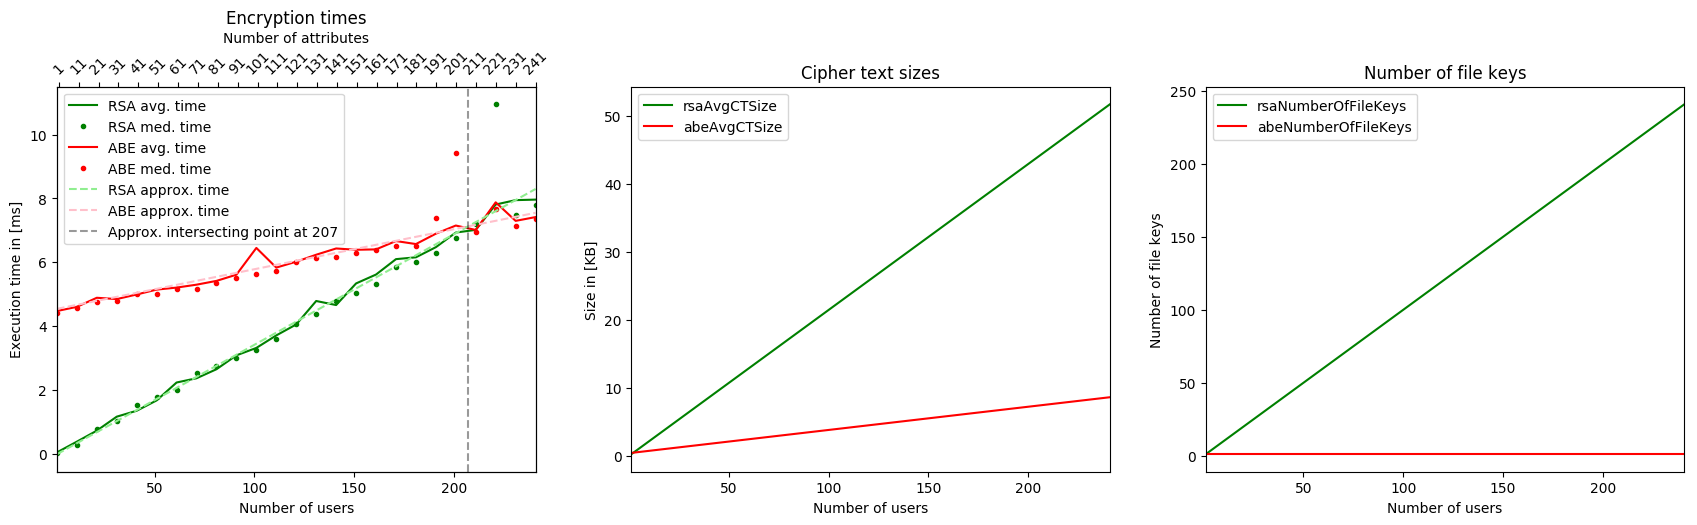
\includegraphics[width=\linewidth]{img/eval-and-policy/encrypt_incrementing_10_attribute_increment_1per1User.png}
    \caption{$1$-for-$1$ configuration using "and"-policy}
    \label{fig:1-for-1-and}
\end{figure}

The configuration of $1$-for-$\infty$ as shown in figure \ref{fig:1-for-infty-and} describes the best-case scenario. Here a group can be completely described by only one attribute regardless of the number of users. \name has an constant overhead since the number of attributes remain constant. The intersecting point can be approximated at $145$ users. From that point on wards \name scales better than the RSA-based approach. With increasing the number of attributes per user, the overhead of \name becomes greater. In the $1$-for-$5$ configuration in Figure \ref{fig:1-for-5-and} the overhead of the prototype has become linear. This is due to additional computations for the increasing number of attributes in the cipher-text. In the configuration of $1$-for-$1$  (Figure \ref{fig:1-for-1-and}), so that each new user introduces a new attribute, the intersecting point gets pushed back to roughly $200$ users. 

Comparing the number of file keys over the increasing number of users, it is observable that the number of file keys indeed scale truly linearly to the number of users in the RSA-based solution. On the other hand, number of file keys remain constant at $1$ for \name when using only "AND"-gates. The cipher text size raises linearly with increasing number of attributes that need to be embedded into this policy. But due to less file keys it still scales better then the RSA based approach. 

\subsubsection{Benchmark: "OR"-Policy}
\begin{figure}[!t]
\centering
    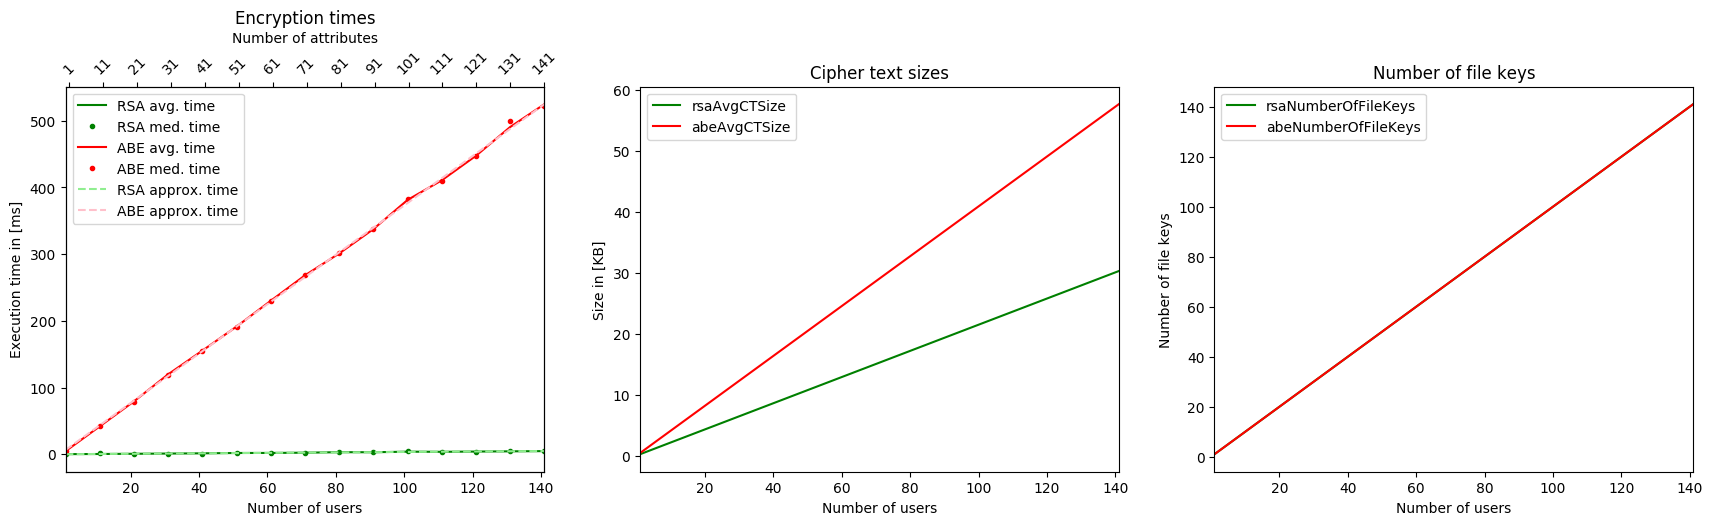
\includegraphics[width=\linewidth]{img/eval-or-policy/encrypt_incrementing_10_attribute_increment_1per1User.png}
    \caption{$1$-for-$1$ configuration using "OR"-policy}
    \label{fig:1-for-1-or}
\end{figure}
\begin{figure}[!t]
\centering
    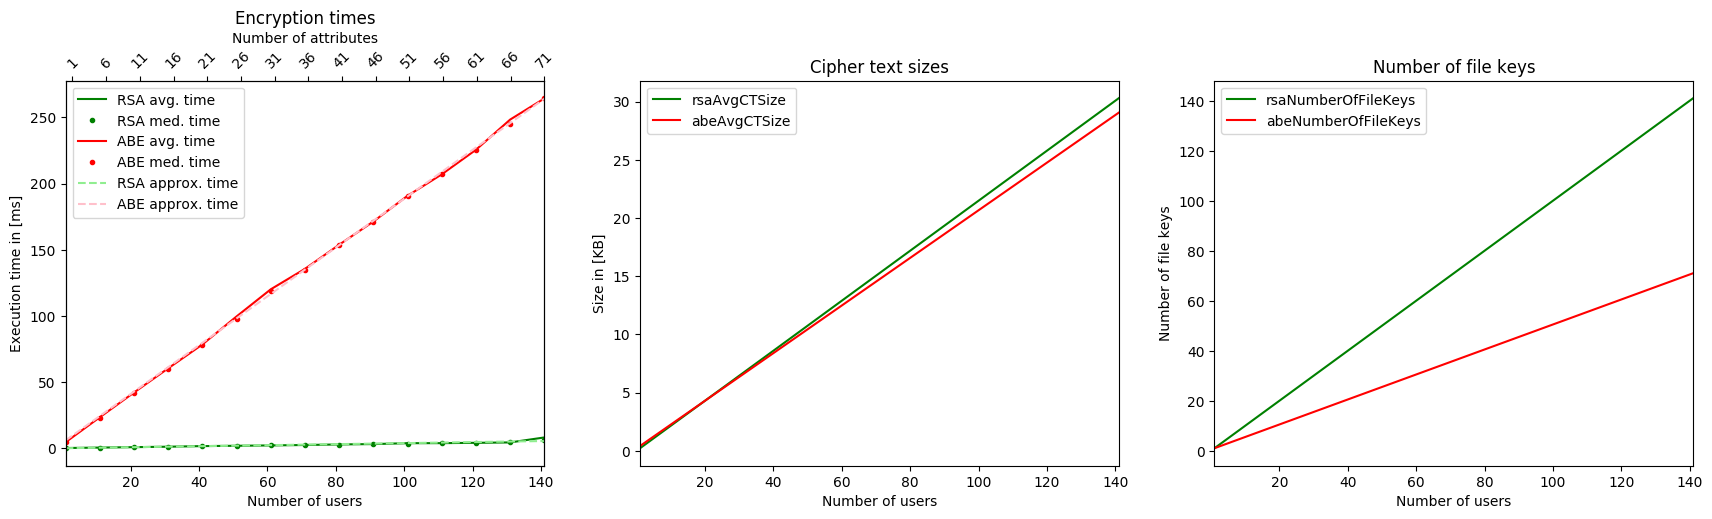
\includegraphics[width=\linewidth]{img/eval-or-policy/encrypt_incrementing_10_attribute_increment_1per2User.png}
    \caption{$1$-for-$2$ configuration using "OR"-policy}
    \label{fig:1-for-2-or}
\end{figure}
\begin{figure}[!t]
\centering
    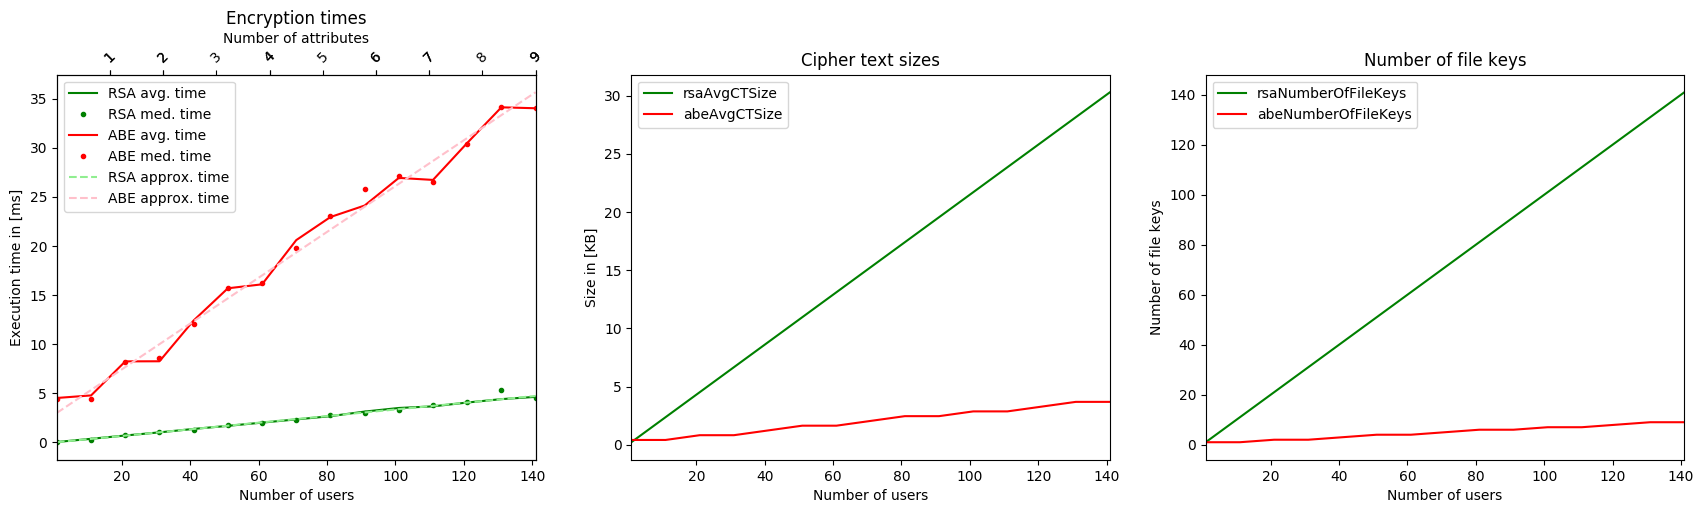
\includegraphics[width=\linewidth]{img/eval-or-policy/encrypt_incrementing_10_attribute_increment_1per16User.png}
    \caption{$1$-for-$16$ configuration using "OR"-policy}
    \label{fig:1-for-16-or}
\end{figure}
\begin{figure}[!t]
\centering
    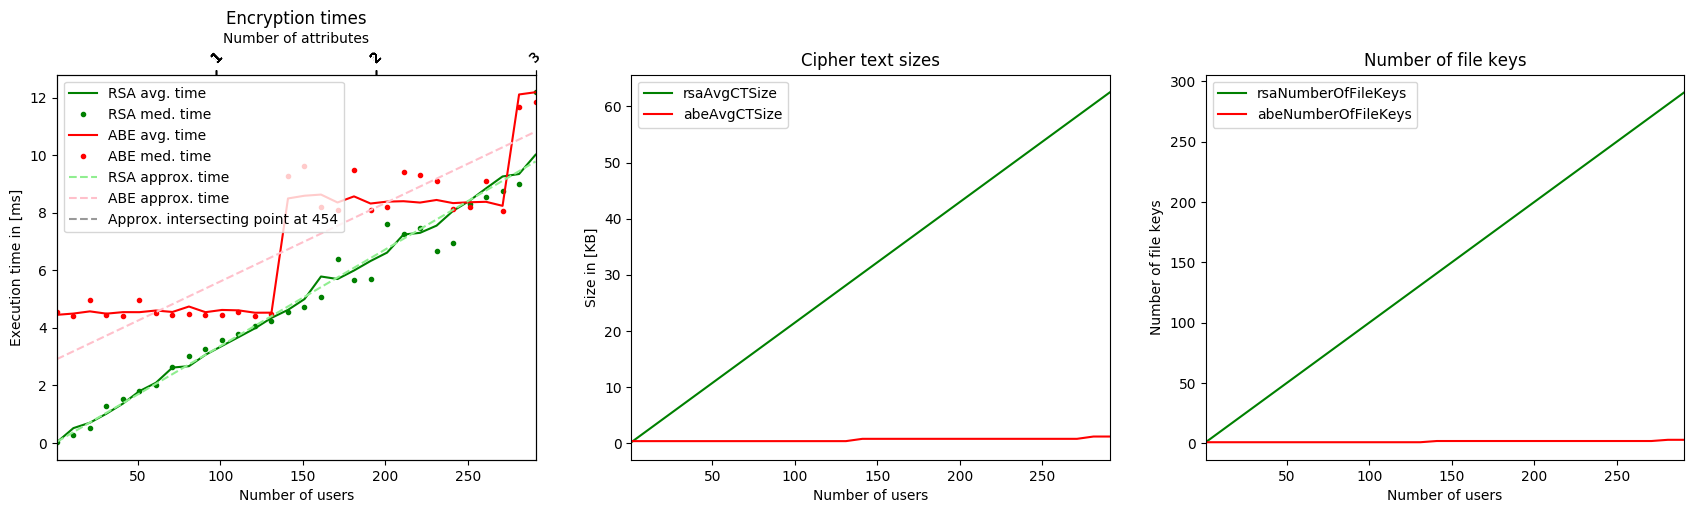
\includegraphics[width=\linewidth]{img/eval-or-policy/encrypt_incrementing_10_attribute_increment_1per140User.png}
    \caption{$1$-for-$140$ configuration using "OR"-policy}
    \label{fig:1-for-140-or}
\end{figure}

Completely different picture is drawn for the benchmark of "OR"-policies. Since for each "OR" a new cipher text needs to be created \name scales with the number of "OR"-gates present in the access policy. This affects execution time, number of file-keys and cipher-text size.


%\begin{figure}[!t]
%\centering
%    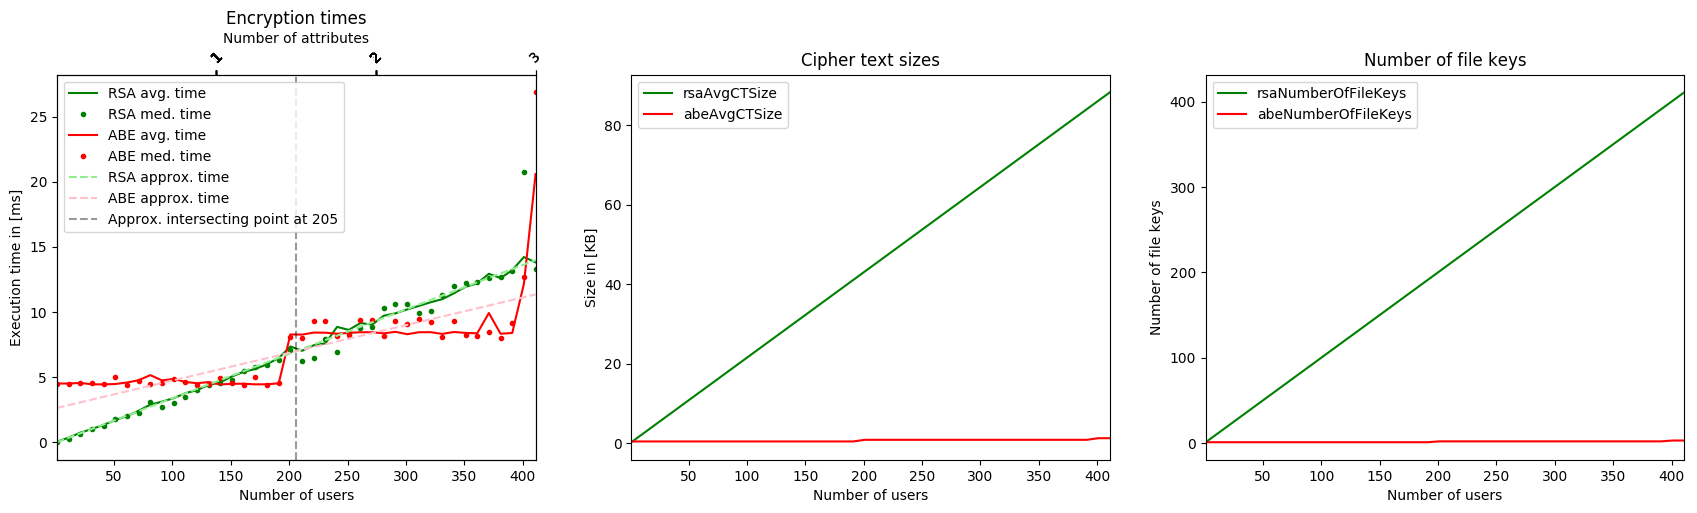
\includegraphics[width=\linewidth]{img/eval-or-policy/encrypt_incrementing_10_attribute_increment_1per200User.png}
%    \caption{$1$-for-$200$ configuration using "OR"-policy}
%    \label{fig:1-for-200-or}
%\end{figure}


Please note that the RSA-based function is the same plot in every figure. The scale and the ABE-plot differs for each figure.  

The worst-case scenario, as introduced in section \ref{sec:upper-bound-and-worst-case-scenario}, is defined as the scenario were the number of users is equal the number of unique attributes combined in an "OR"-policy. This case is shown in figure \ref{fig:1-for-1-or}. In that case is the encryption time of \name two magnitudes higher ($\approx 0ms-550$ms) than the computation time of the RSA-approach ($\approx 0ms-10$ms). Even the cipher text size is substantial greater than the cipher text size per file key. This results from the fact that now, \name scales with the same number of file keys as the RSA approach. No advantage can be gained by the prototype in the worst-case scenario. In general it holds true that the regarding the cipher text size and the number of file keys \name scales better if a group of user can be described by $o < n -1$ "OR" conditions $o$ then there are $n$ users.

As expected, if a configuration of one attribute per two users is used (Figure \ref{fig:1-for-2-or}) the file keys scale twice as good and the cipher text size scale rather similar to the size of the RSA based file keys. 

Reducing the overhead to a 1-for-16 configuration using "OR"-policies, as shown in Figure \ref{fig:1-for-16-or}, a step wise, increasing function is visible in each of the plotted graphics. Each step is directly correlated to another attribute in the access policy.

Finally, in Figure \ref{fig:1-for-140-or}, a configuration was chosen where \name is expected to scale better then the RSA-based approach. Based on that benchmark, the assumption can be extracted that \name scales better regarding computation time if only each 140 users a new OR-gate is introduced in the group access policy.  

\subsection{Member Join}
On member join, in RSA each file key needs to be reencrypted for the new member. That means that each file-key needs to be decrypted using the private key of an existing member and encrypted again with the new members public key. \name has an advantage since it just need to issue the new member the according secret user attribute keys. 

\subsubsection{Expectation}
Based on those facts, it can be assumed that \name scales an constant overhead while the RSA approach scales linearly with the increasing number of cipher texts. While the number of file keys will stay the same for \name, for the reference system they will scale depending on the number of cipher texts linearly. 

\subsubsection{Benchmark: Member Join}
\begin{figure}[!ht]
\centering
    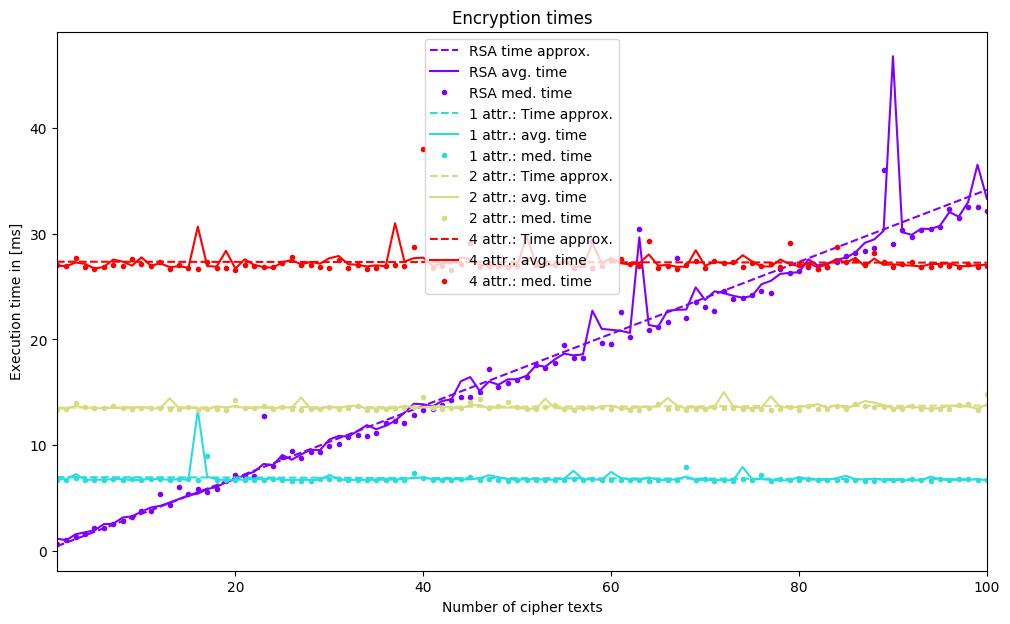
\includegraphics[width=\linewidth]{img/eval-join/join_attr_1.png}
    \caption{Rekeying for one new member. Scaled over the number of attributes}
    \label{fig:member-join}
\end{figure}

Three group configurations were evaluated: On having 1, 2 or 4 attributes respectively. In the benchmark it is assumed that a user need to be issued all of the 1, 2 or 4 attribute secret keys that describe the group to become part of it. As shown in figure \ref{fig:member-join} the previously stated assumptions can be backed. Each of the different \name configurations show a constant overhead. Depending on the number of attributes the intersecting points of 20, 40 and 90 cipher texts can be extracted. After this amount of cipher texts in the group the prototype scales better.

\subsection{Member Leave}
Member-Leave operations comes with a greater overhead for \name. In that scenario, to revoke a member from a group, all of the group attributes need to be revoked from him. That means that for each group attribute, a new attribute private, public and for each non-revoked user an secret update key need to be created by the AA. The secret update keys need to be applied to the secret attribute keys of the non-revoked users. And finally, a cipher text update key needs to be calculated and applied to all cipher texts that contain the revoked attribute to make them accessible to the new attribute key.

The RSA-based approach has an big advantage here: Due to the fact that each file key serves as a unique entry point for a specific user to decrypt the encrypted file, to revoke the user form the group this file key just have to be deleted. 

\subsubsection{Expectation}
The assumption is simply stated that \name does not scale better then the RSA-based approach. Since it scales with the number of attributes that need to be revoked $a_{rev}$, the number of other non-revoked users $u-1$ and the number of cipher texts $c$ we end up with an overhead of $O(a_{rev}(u-1)c)$ which equals a cubic overhead. The reference system is expected to just scale linearly with the number of cipher texts. 

\subsubsection{Benchmark: Member Leave}
\begin{figure}[!ht]
\centering
    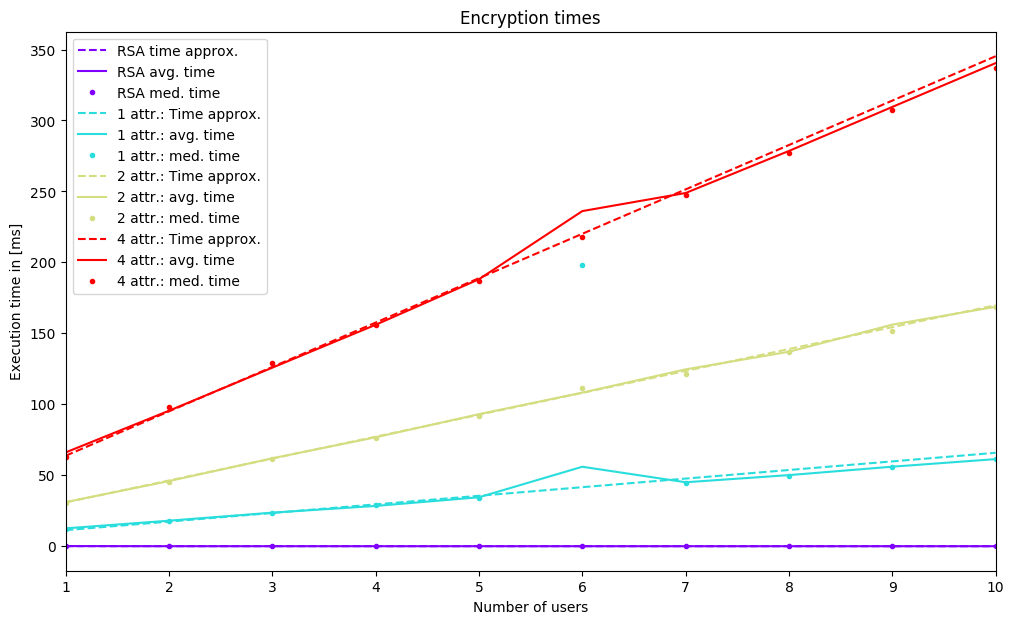
\includegraphics[width=\linewidth]{img/eval-leave/leave_attr_1_users_2.png}
    \caption{One member leaves the share. Scaled over the number of attributes}
    \label{fig:member-leave}
\end{figure}

Figure \ref{fig:member-leave} shows the exact expected behavior. For already one cipher text the gab between the different number of attributes and the RSA-based approach is clearly notable. \name is magnitudes slower than the RSA-based approach.

In a real world system the cipher text and the user secret key update would happen on the server and client device side respectively. Further, the application of the update key to the secret keys or cipher texts can happen in parallel to further speed-up this process. In the end \name scales much worse since it comes with unneglectable more overhead. 

\section{Summary}
The previous performance and scalability analysis strengthen the thesis that \name scales better than the reference implementation of the classical RSA-based sharing scheme. It was shown that in the worst-case scenario the same number of file-keys where produced and in the best-case scenario only one file-key need to be maintained. While the number of file-keys are certainly an issue, the size of the resulting file-keys need to be respected as well. The proposed ABE-based solution consumes, due to additional meta information, such as the access policy and data owner references, a much more storage per file-key. Calculating this into account \name archives its goal of consuming less file-key storage if a group can be described by $n/2$ conditions combined using "ORd-gates (see figure \ref{fig:1-for-2-or} for reference).

In the end it boils down to the access policy a user chooses. If this policy is constructed in an excluding fashion (using only or mostly "AND"-gates)  \name scales better in the long-term. But if to much attributes are used in the access policy many cipher-texts need to be updated each time a user or attribute gets revoked from the system. 

